\documentclass{IEEEtran}
\usepackage[utf8]{inputenc}
\usepackage{acronym}
\usepackage{footnote}
\usepackage{algorithmic}
\usepackage{graphicx}
\usepackage[autostyle=true,german=quotes]{csquotes}

\usepackage{hyperref}

\long\def\comment / *#1* /{}


\begin{document}


\title{cowbus -- a small home automation bus}
\author{Robin~Backhaus \and Patrick~Kanzler \and Josef~Schnurrer \and Michael~Zapf}
\date{\today}



\maketitle

\begin{abstract}
    TODO
\end{abstract}


\section{Einleitung}

    \enquote{Smart Home} ist ein Schlagwort, um das man im 21. Jahrhundert
    kaum noch herum kommt. Der moderne Mensch möchte sein Zuhause vernetzen.
    Lichtschalter sind nicht mehr nur noch passive Komponenten in einer
    Elektroinstallation, sie sind aktive Kommunikationspartner in einem großen Netz.

    Das Licht wird nicht nur am Schalter, sondern bequem von der Couch aus mit dem
    Smartphone geschalten, eingehende E-Mails erscheinen nebenbei im Fernsehbild,
    die Verdunklung fährt automatisch herunter sobald die Sonne blendet --
    all das ist keine Science Fiction mehr sondern längst Realität.

\section{Motivaton}

    Die meißten erhältlichen \enquote{Smart Home}-Lösungen sind teuer und nicht offen.
    Da die Beliebtheit solcher Systeme immer größer wird, wäre eine größere 
    Zugänglichkeit durch günstige Alternativen und langfristige Sicherheit, 
    sowie mehr Kontrolle für und durch den Anwender wünschenswert.
    Unser Fokus liegt daher auf modernen, offenen Standards und einer drahtlosen, 
    flexiblen und damit einfach zu erweiternden Netzwerktopologie.
    Mit möglichst günstigen Komponenten sollen dabei Sensoren und Aktoren 
    mit verschiedensten Funktionen ermöglicht werden.
    Eine Anknüpfung an vorhandene IP-basierende Netze durch Gateways würde die 
    Anwendungsmöglichkeiten zusätzlich erhöhen 
    und es ermöglichen bereits bestehende und neue externe Anwendungen mit dem 
    cowbus zu verbinden.

\section{Projektziele und Ideen}

    An zentraler Stelle des Projektes steht die Kommunikation zwischen den 
    Netzwerkknoten und ein Netzwerkmodell, dass möglichst flexibel erweiterbar 
    und verkleinerbar sein soll.
    Dazu wird ein drahtloses Mesh-Netzwerk mit dezentraler Organisation implementiert 
    und an Beispiel-Sensoren und -Aktoren getestet. Optional könnte nach ersten 
    Funktionstests der ausgewählten Hardware oder im Anschluss an die erfolgreiche 
    Implementierung eines Netzwerkes der Standart \enquote{6LoWPAN} implementiert werden. 
    Als dritte Komponente neben Aktoren und Sensoren soll ein Ethernet-Gateway 
    implementiert werden. Als optionales Anwendungsbeispiel würde sich \enquote{OpenHAB} 
    besonders eignen.

\section{Projektablauf und Meilensteine}

    \section{Konkretisierung der Ziele und Projektplanung}

        TODO: aus Blogbeitrag Brainstorming und Projektbeginn

    \subsection{Kennenlernen von RIOT OS}

        \url{http://www.riot-os.org/} \enquote{The friendly Operating System for the 
        Internet of Things.}, Multithreading, gut portierbar (Schichtenarchitektur), 
        Lizenz: LGPLv2

    \subsection{Funkchip nrf24l01+}

        2,4 GHz (ISM-Band), bis zu 2 Mbps, handliches Modul

    \subsection{Erstes Prototyping mit Discovery Boards}



    \subsection{Erste Funkübertragung und Messung der Funkreichweite}



    \subsection{ARM Cortex M0: STM32F030C8T6}

        bis zu 48 MHz, Gehäuse LQFP48 (7x7 mm)

    \subsection{Platinendesign}

        RGB-LED, Batterie-/Akkubetrieb oder USB, drei Taster, Board ca 4 cm Radius

    \subsection{Zwischenpresentation}
    

\section{Verwendete Programmiersprachen und Techniken}

\section{Verwendete Software und Hilfsmittel}

    GitHub, KiCad
\section{Aufgetretene Hindernisse und Risiken}

\section{Systemaufbau}
    TODO

    \subsection{Funkmedium}
        Als Übertragungsmedium kommt eine $2,4GHz$-Technologie
        zum Einsatz. Eine Funktechnologie eignet sich besonders gut dazu
        bereits bestehende Installationen um intelligente Komponenten
        zu erweitern, ohne größere bauliche Änderungen vornehmen zu müssen.

        Die Wahl eines ISM-Frequenzbandes (\enquote{Industrial, Scientific and Medical Band})
        ist in erster Linie bedingt durch die gute Verfügbarkeit von günstigen
        Systemkomponenten und der weltweiten Einsetzbarkeit ohne Anpassung der
        genutzten Frequenzen.

        Genutzt wird der Funkkanal im Moment als Broadcastmedium.
        Jeder Knoten kann also prinzipiell jedes Paket sehen und verarbeiten.
        Dies spart für den Anfang sehr viel Logik und Routingaufwand,
        da Pakete einfach ins Netz geflutet werden können und der entsprechende
        Empfänger (wobei das durchaus mehrere Knoten sein können -- ein Schalter
        könnte beliebig viele Lampen schalten) selbst an der Adresse erkennen
        kann, dass er darauf reagieren muss.

    \subsection{Komponenten}
        Grundsätzlich besteht der cowbus aus drei Typen von Komponenten,
        die auch in Abb. \ref{fig:comp} schematisch dargestellt sind.

        \begin{figure}
            \centering
            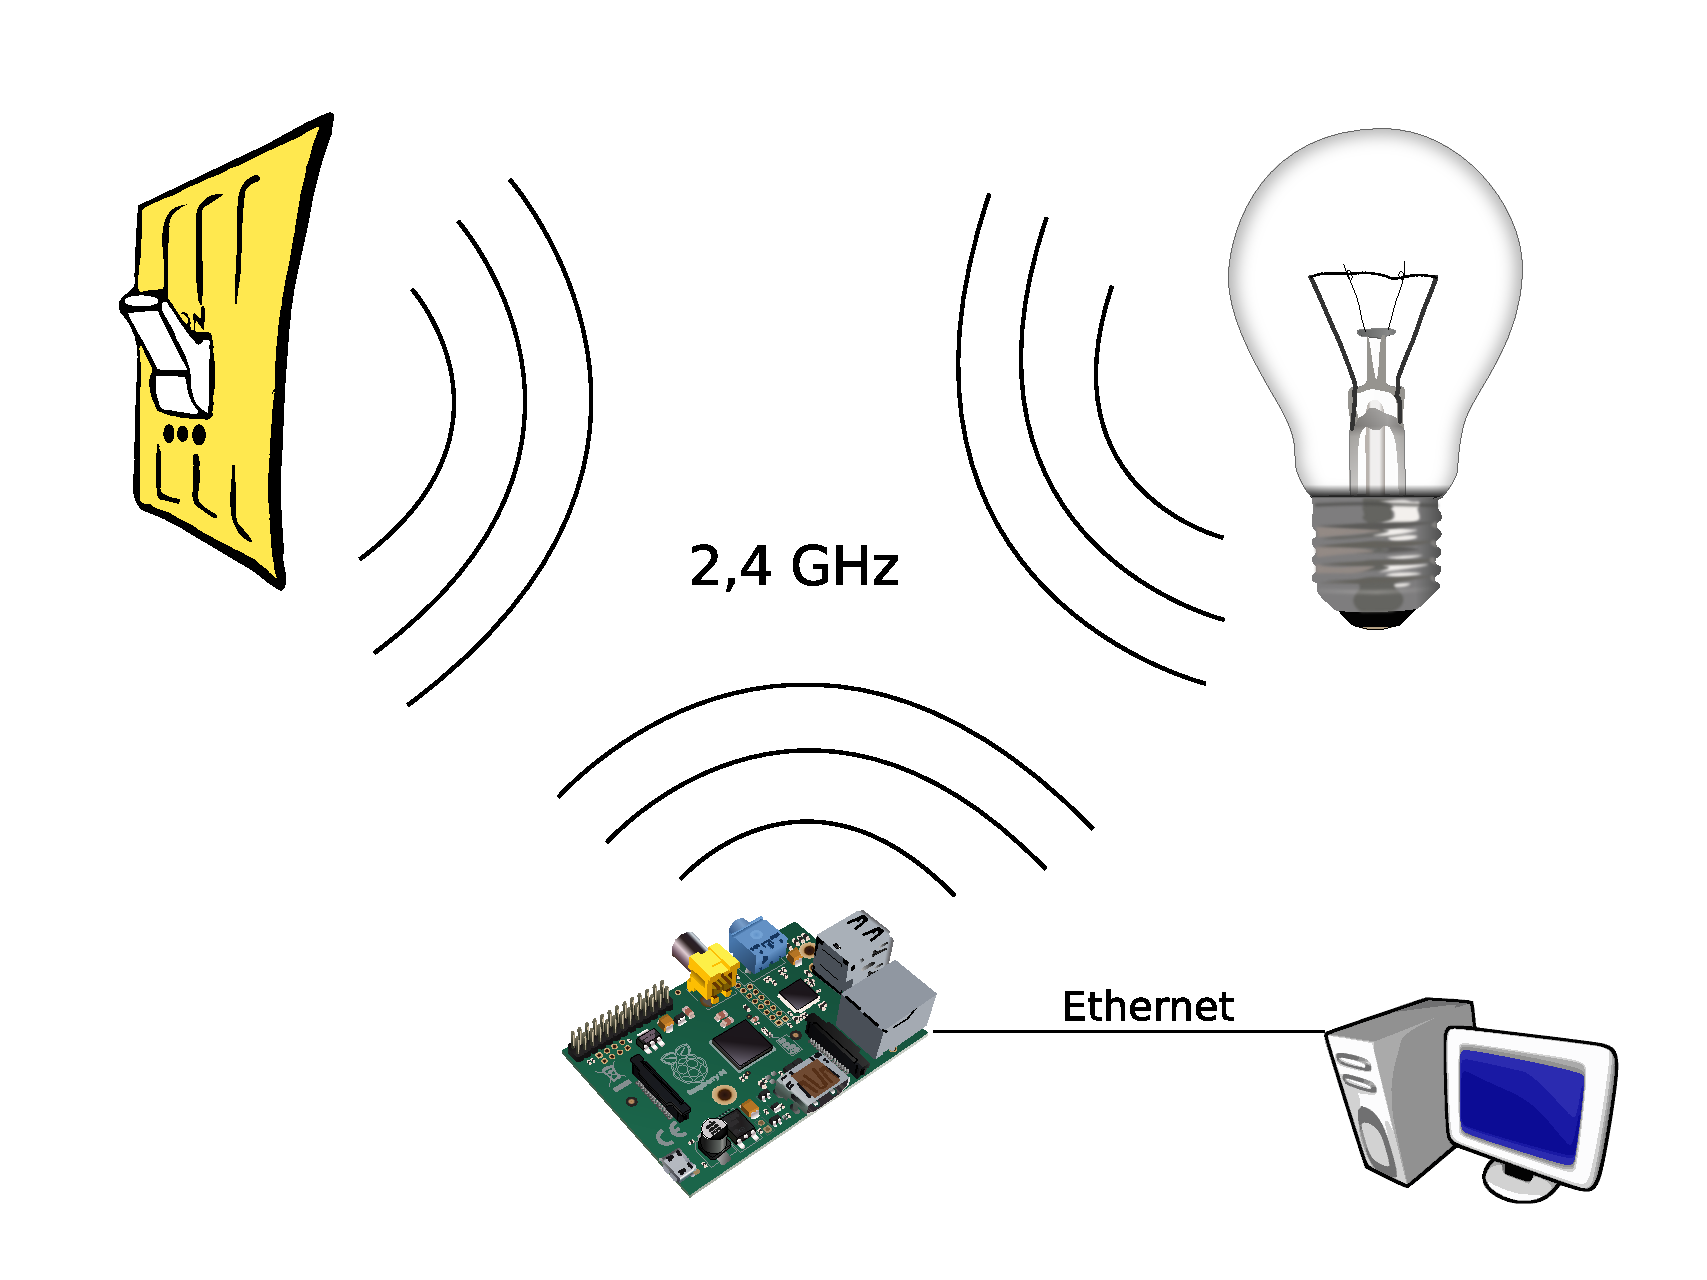
\includegraphics[width=0.5\textwidth]{img/system}
            \caption{Schematische Darstellung der beteiligten Komponententypen}
            \label{fig:comp}
        \end{figure}

        \subsubsection{Sensorknoten}
            Sensorknoten sind aus Sicht des Systems im aktuellen Entwurf
            zunächst \enquote{dumm}. Sie enthalten keinerlei Wenn-Dann-Logik
            sondern produzieren ausschließlich Nachrichten mit bestimmten
            Aussagen, z.B. \enquote{Ich bin Knoten A und meine erste Taste
            wurde gedrückt}.
        \subsubsection{Aktorknoten}
            Aktorknoten ist die eigentliche Aktion-Reaktion-Logik eingepflanzt.
            Sie lauschen auf dem Kommunikationsmedium und warten auf Anweisungen
            ihre möglichen Aktionen auszuführen.

            Dabei sind zwei Varianten vorgesehen:
            \begin{itemize}
                \item Ein Aktor kann eine Nachricht mit seiner eigenen Adresse
                    erhalten. Das bedeutet für ihn, er soll diese Aktion
                    ausführen, unabhängig davon wer das Ereignis ausgelöst hat.
                \item Ein Aktor kann programmiert werden auf bestimmte andere
                    Adressen und Nachrichten zu reagieren.
                    So kann beispielsweise eingestellt werden, dass ein Aktor
                    dann schaltet, wenn er eine Nachricht entdeckt, in der steht
                    \enquote{Ich bin Knoten A und meine erste Taste
                    wurde gedrückt} (siehe oben).
            \end{itemize}

            Durch diese zwei Varianten ist es auf der einen Seite möglich
            dezentral Nachrichten auszulösen und darauf zu reagieren, wobei
            die Auslöser, also die Sensoren selbst relativ einfach aufgebaut
            sein können. Die aufwändigere Logik, welcher Sensor welche Aktion
            auslöst, kann im Aktor implementiert werden.
            Auf der anderen Seite ist es aber trotzdem möglich, das System
            zentral zu nutzen, indem Sensornachrichten von einem zentralen
            Punkt empfangen werden, der anschließend Nachrichten mit konkreten
            Aktoradressen versendet. So können auch Aktoren \enquote{dumm}
            bleiben und können (z.B. in einem sehr kleinen, temporären Aufbau)
            ohne jede Programmierung verwendet werden, ohne dass sie von den
            konkreten Sensoren wissen müssen.

            Wie ein solches Gateway aussehen könnte zeigt der folgende Abschnitt.

        \subsubsection{Gateway (im Moment der PI)}
            Ein System, dass unabhängig von äußeren Steuerungsinfrastrukturen
            funktionieren kann, ist für die Akzeptanz im Gebäude wichtig.
            Wenn kein Lichtschalter im Haus mehr funktioniert, weil
            im Keller jemand das falsche Netzwerkkabel gezogen hat,
            wird kein Nutzer recht überzeugt sein.
            Umgekehrt ist es allerdings auch wichtig, Schnittstellen zu
            etablierten Kommunikationsstrukturen zu bieten.
            So ist eine Anbindung an vorhandene IPv4- oder IPv6-Netze
            wünschenswert, sodass auch mächtigere Komponenten integriert werden
            können, die unter Umständen noch weitere Kommunikationsmöglichkeiten
            bieten.

            Momentane Lösung dieses Wunsches ist die Integration eines Computers
            in den cowbus. Die offensichtlichste Möglichkeit war auch bei diesem
            Projekt ein Raspberry PI \footnote{\url{http://www.raspberrypi.org/}},
            der bereits alle nötigen Schnittstellen mitbringt, um direkt das
            $2,4-GHz$-Funkmodul und das vorhandene \ac{LAN} anzuschließen.

            Auf dem Raspberry PI läuft ein kleiner in C++ verfasster Daemon.
            Dieser steuert zum einen das Funkmodul und wartet auf Pakete aus
            dem Funknetz.
            Auf der anderen Seite enthält er einen kleinen Websocket-Server,
            über den von jedem beliebigen PC, der ihn über das \ac{LAN}
            erreichen kann, Pakete in das Funknetz verschickt und aus diesem
            empfangen werden kann.

            Dazu steht eine kleine HTML/JavaScript-Anwendung zur Verfügung,
            die in jedem modernen Browser läuffähig sein sollte.


    
    \subsection{Paketaufbau}

\section{Knoten-Prototyp-Hardware}
*Wahl des Prozessors

*Wahl fiel auf STM, weil 8bit zu wenig Dampf hat, ARM hat solide Toolchain

*weiterer Vorteil: Discovery-Boards günstig, um sofort mit der Entwicklung anzufangen



*parallel dazu Entwicklung richtiger Hardware

*Anforderungen:

*Idee: Schaltermodul, welches in eine Unterputzdose passt --> bedingt Form

*möglichst günstig

*...



*

    Platine, Aufbau, Designentscheidungen, ...


\section{Software und System}
    \subsection{Kommunikationsstruktur: Nachrichtenbasiert, jeder Knoten entscheidet anhand Adresse ob er interessiert ist am Inhalt}
    \subsection{RIOT - Was, Warum; evtl. auch kritische Auseinandersetzung?}

\section{Ausblick}
Was geplant ist: CSMA/CA, ...;
kritische Auseinandersetzung mit getätigten Design-Entscheidungen

\section{Zusammenfassung}



\section*{Abkürzungen}
\renewcommand{\IEEEiedlistdecl}{\IEEEsetlabelwidth{CSMA/CA}}
\begin{acronym}
    \acro{CSMA/CA}{Carrier Sense Multiple Access with Collision Avoidance}
    \acro{LAN}{Local Area Network}
\end{acronym}
\renewcommand{\IEEEiedlistdecl}{\relax}% remember to reset \IEEEiedlistdecl


\comment / *
\listoffigures
\clearpage

\listoftables
\clearpage
* /

\nocite*
\bibliographystyle{IEEEtran}
\bibliography{IEEEabrv,projektdoku_cowbus}

\end{document}
